\subsection{Registros de interés}
\subsubsection{Registro DDRx - Data Direction Register.}
En este registro n puede ir desde A, B o D. Este registro sirve para establecer si los pines son de entrada o salida. Se pone en el pin de interés un 1 para salida y un 0 para entrada. A continuación se presenta un ejemplo para el registro DDRB \cite{datasheet}.

\begin{figure}[H]
\centering
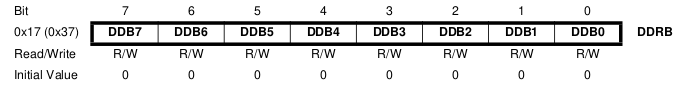
\includegraphics[scale=0.9]{./images/DDRB.png} 
\caption{Diagrama de registro DDRB \cite{datasheet}.}
\label{f1}
\end{figure}


\subsubsection{Registro PORTx - Data Register}
En donde x de igual forma puede ir de A, B o D. Permite escribir información o los datos como tal en los pines. Puede tomar valores de 0 o 1. \footnote{Si este registro estuviera configurado como entrada y se escribe un 1 en el bit correspondiente de este registro entonces se activa la resistencia interna Pull-Up; para apagarla debe configurarse el pin como salida.} A continuación se muestra un ejemplo para el registro PORTB \cite{datasheet}.
\begin{figure}[H]
\centering
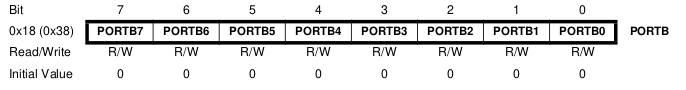
\includegraphics[scale=0.9]{./images/PORTB.png} 
\caption{Diagrama de registro PORTB \cite{datasheet}.}
\label{f1}
\end{figure}

\subsubsection{Registro GIMSK - General Interrupt Mask Register}
Permite habilitar y deshabilitar interrupciones. Habilitando estos registros entonces ya se puede hacer uso de las funciones de interrupciones \cite{datasheet}.

\begin{figure}[H]
\centering
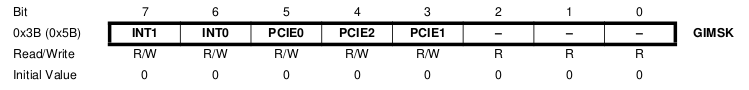
\includegraphics[scale=0.9]{./images/GIMSK.png} 
\caption{Diagrama de registro GIMSK \cite{datasheet}.}
\label{f1}
\end{figure}

\subsubsection{Registro MCUCR - MCU Control Register}
Permita la manera en la que se habilitan las interrupciones, ya sea por flanco creciente o decreciente \cite{datasheet}.
\begin{figure}[H]
\centering
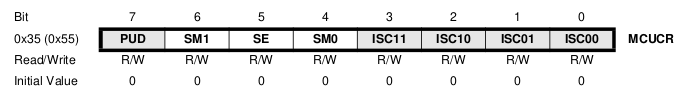
\includegraphics[scale=0.9]{./images/MCUCR.png} 
\caption{Diagrama de registro MCUCR \cite{datasheet}.}
\label{f1}
\end{figure}

\subsubsection{Registro TCCR0x}
en donde x puede ser A o B.
Permite configurar el modo de operación para la utilización de timers. Más específicamente permite modificar el prescaler de los timers A continuación se presenta un ejemplo del diagrama para el registro TCCR0A.  \cite{datasheet}.
\begin{figure}[H]
\centering
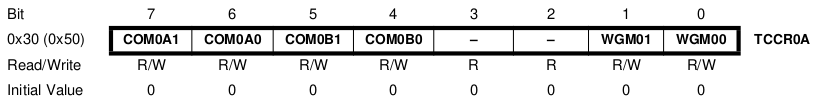
\includegraphics[scale=0.8]{./images/TCCR0A.png} 
\caption{Diagrama de registro TCCR0A. \cite{datasheet}.}
\label{f1}
\end{figure}